\clearpage
\chapter{\textbf{Lokalisierung - Lösungsansätze}}\label{chap:Lokalisierung - Lösungsansätze}
\addtocontents{toc}{\vspace{0.8cm}}
%TODO einleitung lokalisierung schreiben --> position tracking, global lokalisation, kidnapping recovery
einleitende worte

\section{Monte Carlo Localization}\label{sec:mcl}
\addtocontents{toc}{\vspace{0.8cm}}

% TODO Kapitel Monte Carlo Lokalisierung schreiben
Der von Daeller et al. \cite{Monte-Carlo-Localization} entwickelte \textit{Monte Carlo Localization} (MCL) Lokalisierungsalgorithmus verfolgt das Ziel einen mobilen Roboter in bekannter Umgebung zu orten. Der Algorithmus bekommt eine 2D Occupancy Grid Map, das Motion-Model und das Oberservation-Model des Systems zur Verfügung gestellt, generiert damit eine geschätzte 2D Position und ist in der Lage sowohl Position-Tracking, Globale Lokalisierung, als auch Kidnapping-Recovery zu absolvieren. \\
Es handelt sich hierbei um einen Partikelfilter, bei dem jedes Partikel eine mögliche Position des mobilen Systems ohne Toleranz darstellt. Die Einschätzung der Position $Bel(l)$ wird dargestellt durch ein \textit{N}-zahliges Set von gewichteten, zufälligen Partikeln oder \textit{Samples}.Ein Sample kann dargestellt werden durch $s=\langle\langle x,y,\psi \rangle,p\rangle$, wobei die $\langle x,y,\psi$ die Position, und $p$ das Gewicht beziehungsweise die Wahrscheinlichkeit dieser Position repräsentiert. Das Vorgehen ist eingeteilt in die Schritte \textbf{Robot Motion} und \textbf{Sensor readings}. Folglich wird der Algorithmus beginnend mit dem Schritt \textbf{Sensor readings} erläutert.\\
Im Beispiel \ref{fig:mcl} wird die eindimensionale Position eines mobiler Roboter berechnet, indem er auf einer Geraden an mehreren Türen entlang fährt. Ein außen montierter Sensor gibt an, ob er sich an einer Tür befindet. Zum Zeitpunkt der Intialisierung des Algorithmus wird das erste Set an Samples mit vollkommen willkürlichen Positionen, und dem Gewicht $p=N^{-1}$ generiert. Dann folgt der Schritt Sensor readings \ref{fig:s_mcl_sensor} wird das Observation-Model genutzt um die Umgebung wahrzunehmen, und von jedem individuellen Sample aus zu berechnen wie wahrscheinlich die erhaltene Messung an der Position \textit{l} des Samples ist. Die Gewichtungen $p$ der einzelnen Samples in dem Sample-Set werden dann entsprechend der Ergebnisse angepasst, sodass $\sum_{n=1}^{N} p_n =1$ gilt. Je wahrscheinlicher die reale Messung am Ort des Samples ist, desto höher ist dessen Gewichtung.
\mbox{}
\begin{figure}\label{fig:mcl}
  \begin{subfigure}[t]{.5\textwidth}
    \centering
    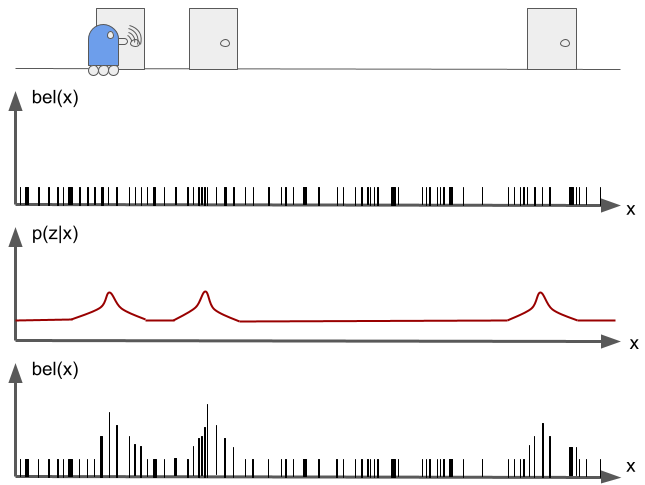
\includegraphics[width=.8\linewidth]{pic/loesungen/1a_mcl.png}
    \caption{Sensor readings}
    \label{fig:s_mcl_sensor}
  \end{subfigure}\hfill
  \begin{subfigure}[t]{.5\textwidth}
    \centering
    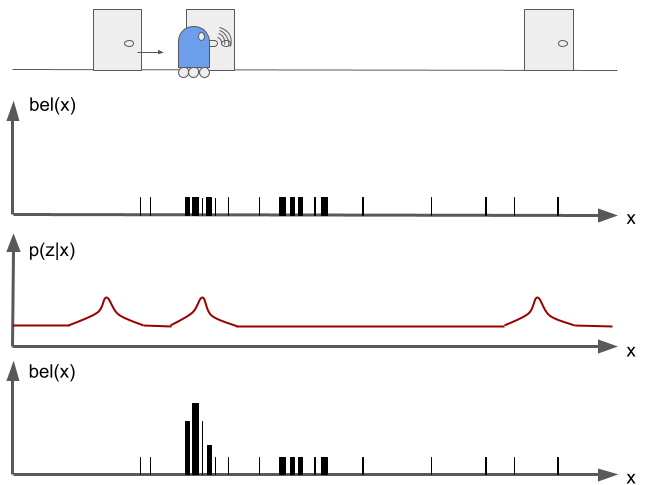
\includegraphics[width=.8\linewidth]{pic/loesungen/1b_mcl.png}
    \caption{Robot Motion}
    \label{fig:s_mcl_motion}
  \end{subfigure}
\end{figure}
\mbox{}
\\Es folgt der Schritt Robot Motion \ref{fig:s_mcl_motion}: Der Roboter bewegt sich, der Algorithmus generiert ein neues Set mit $N$ neuen Samples, die mithilfe des Motion-Models die neue Position nach der Bewegung annähern. Dafür werden per Zufallsverfahren Samples aus dem vorherigen Set entnommen gegebenenfalls vervielfacht und jedes Gewicht durch $N^{-1}$ ersetzt. Zusätzlich werden dem Set ein wenig neue Samples mit willkürlich generierten Positionen hinzugefügt. Das hilft dem System dabei sich im Falle eines Kidnapping-Szenarios neu zu lokalisieren. Anschließend macht der mobile Roboter wieder Gebrauch von seinem Observation-Model und führt den Schritt Sensor readings wieder aus. Das Partikel mit dem zuletzt höchsten Gewicht stellt die aktuelle Position des Roboters dar. Je mehr Iterationen durchgeführt werden, desto näher befinden sich die Partikel beieinander und desto genauer wird die angenäherte Position.

\subsection{AdaptiveMonte Carlo Localization}\label{subsec:mcl_surfel}
\addtocontents{toc}{\vspace{0.8cm}}
% TODO Unterkapitel AMCL


\subsection{Monte Carlo Lokalisierung mit Surfel Grid Maps}\label{subsec:mcl_surfel}
\addtocontents{toc}{\vspace{0.8cm}}
% TODO Unterkapitel MCL mit Surfel Grid Maps schreiben


\subsection{Dreidimensionale Indoor Lokalisierung}\label{subsec:}
\addtocontents{toc}{\vspace{0.8cm}}
% TODO Unterkapitel 3D Indoor Lokalisierung schreiben